\section{First numerical calculation and validation}

We solved the Rayleigh--Lamb equations for a representative isotropic aluminum
plate with $d=1\,\mathrm{mm}$, $\rho=2700\,\mathrm{kg/m^3}$,
$c_L=6320\,\mathrm{m/s}$, and $c_T=3130\,\mathrm{m/s}$. The nondimensional
grid covered $0.04\le kh\le8$ and $0<\omega h/c_T\le12$.
Figure~\ref{fig:dispersion} shows the first three roots of each symmetry family.

\begin{figure}[htbp]
  \centering
  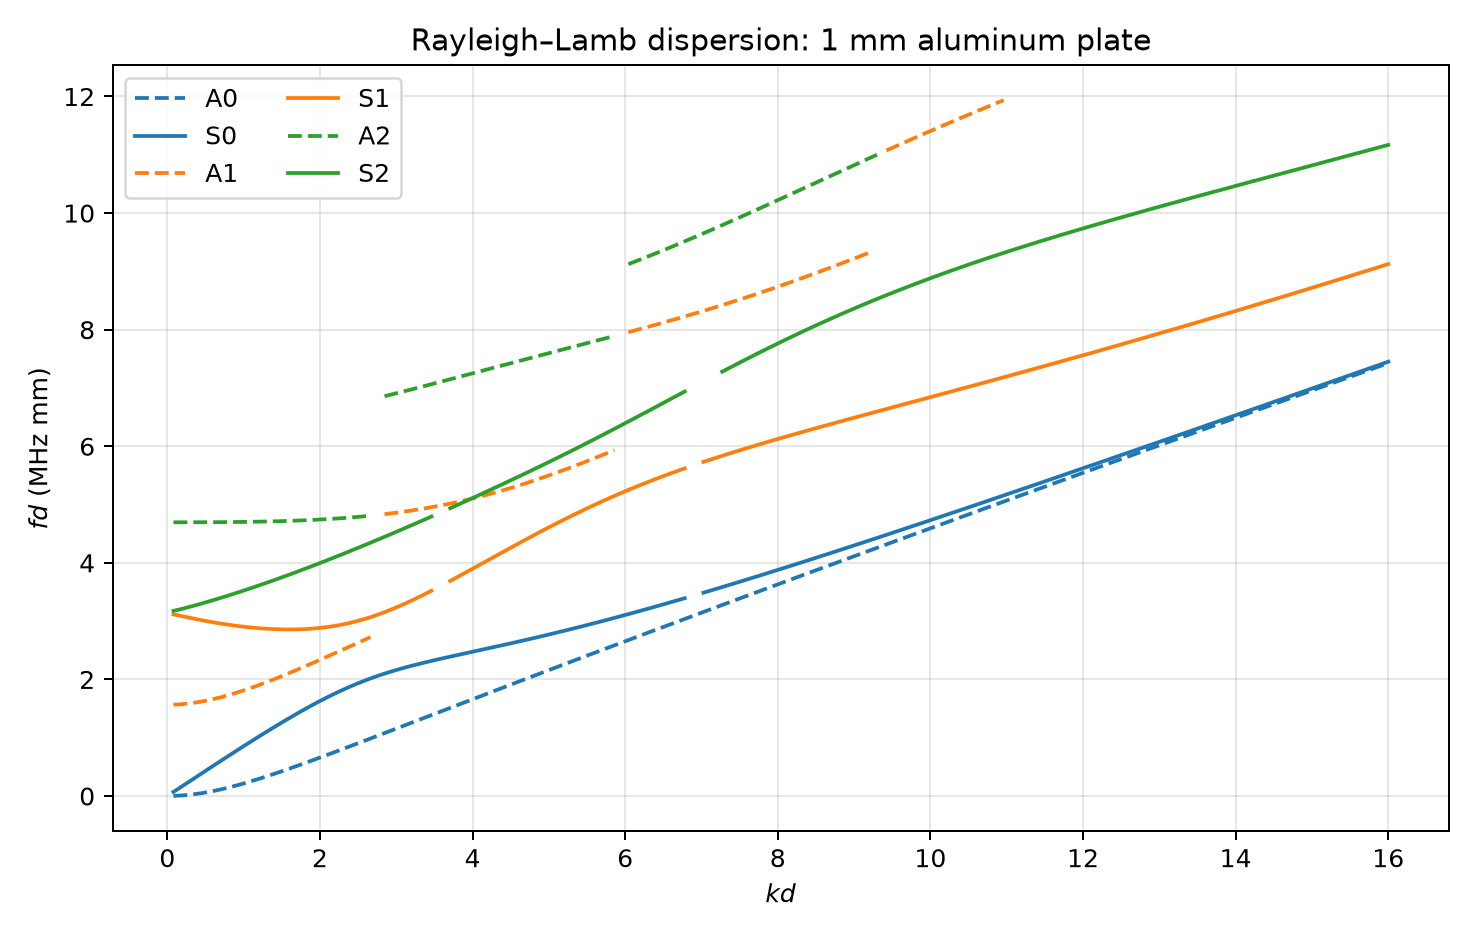
\includegraphics[width=0.92\linewidth]{results/dispersion.png}
  \caption{Calculated Rayleigh--Lamb dispersion curves. Solid lines denote
  symmetric roots and dashed lines antisymmetric roots.}
  \label{fig:dispersion}
\end{figure}

The first symmetric higher-order branch has a local minimum at
\begin{equation}
 kh=0.7989,\qquad fd=2.8568\ \mathrm{MHz\,mm},
\end{equation}
the first ZGV candidate in the sampled range. At low frequency, the $S_0$ branch
agrees with the plane-stress plate velocity to a median relative error of
$0.011\%$; $A_0$ agrees with the Kirchhoff--Love flexural limit to $0.150\%$.
The maximum normalized characteristic residual is $2.44\times10^{-9}$. Halving
the frequency scan density changes the nondimensional roots by no more than
$3.25\times10^{-12}$ after removable bulk-wave-threshold roots are excluded.

For the causal example we selected $A_0$ at $kh\simeq1$, giving
$f=0.6519\,\mathrm{MHz}$. The normalized source was a Gaussian line of width
$1\,\mathrm{mm}$, the observation distance was $20\,\mathrm{mm}$, and
$\gamma/\Omega=0.01$. To represent a frequency-filtered measurement, the modal
integral retained frequencies between $0.5\Omega$ and $1.5\Omega$.

\begin{figure}[htbp]
  \centering
  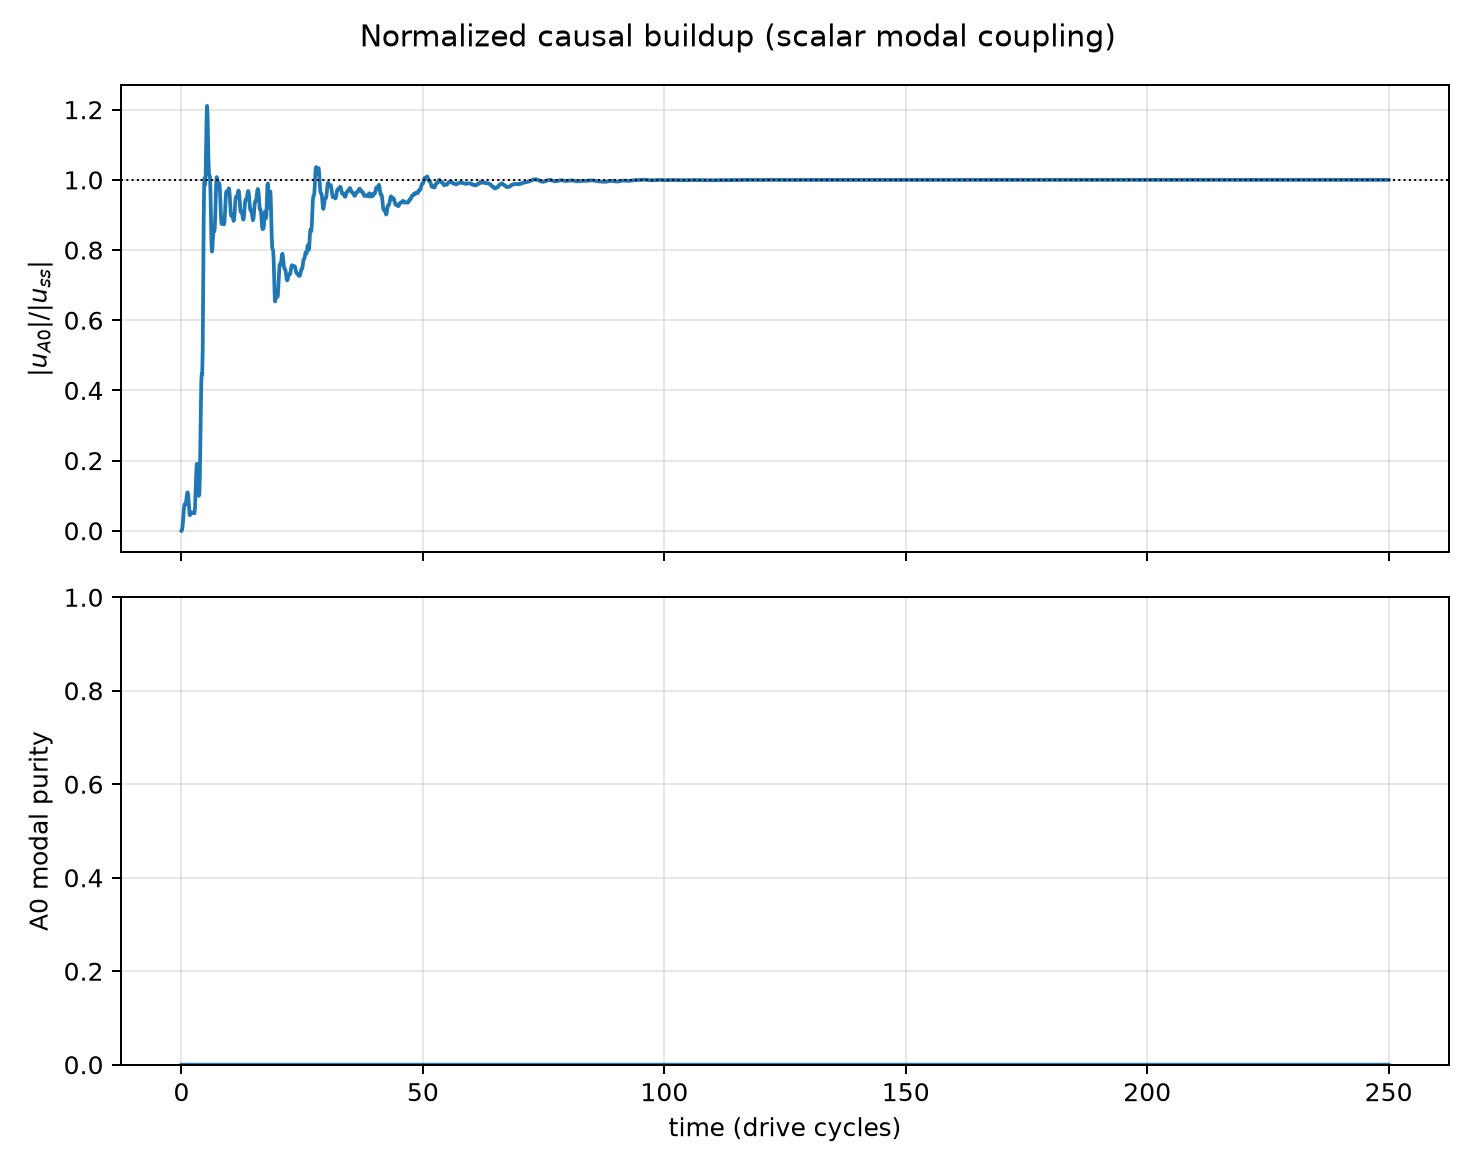
\includegraphics[width=0.92\linewidth]{results/causal_buildup.png}
  \caption{Normalized causal buildup and modal purity. Absolute amplitude is
  not implied because full thermoelastic eigenmode overlaps are not yet used.}
  \label{fig:buildup}
\end{figure}

The group-delay estimate is $x/|v_g|=6.58\,\mu\mathrm{s}$, whereas the transient
envelope remains below $5\%$ of the steady harmonic amplitude only after
$76.39\,\mu\mathrm{s}$, approximately 50 drive cycles. Halving the time step
changes the result by $0.05$ cycle. A 27-case sweep over distance, Gaussian
width, and damping gives an $N_{95}$ proxy from 24 to 117 cycles. The calculation
therefore demonstrates the distinction between arrival and settling, but is not
yet an absolute experimental prediction.

\paragraph{Reproducibility and scope.}
The complete calculation is in \texttt{calculations/run\_all.py}; it writes the
data, figures, parameter sweep, and validation report to \texttt{results/}. The
oscillator solution satisfies zero initial displacement and velocity to machine
precision. Absolute predictions still require normalized Lamb eigenfields, an
optical absorption profile, and a calibrated attenuation law.
